Ring signatures, introduced by Rivest, Shamir and Tauman, \cite{AC:RivShaTau01}, allow to anonymously sign a message on behalf of a ring of users $P_1,\ldots,P_n$, only if the signer belongs to that ring. Although there are other cryptographic schemes that provide similar guarantees (e.g.~group signatures \cite{EC:ChaVan91}), ring signatures are not coordinated: each user generates secret/public keys on his own -- i.e.~no central authorities -- and might sign on behalf of a ring without the approval or assistance of the other members.

While the more efficient constructions have signature size logarithmic in the size of the ring \cite{EC:GroKoh15,EC:LLNW16}, all of them rely on the {random oracle model}.
Without random oracles all constructions have signatures of size linear in the size of the ring, being the sole exception the $\Theta(\sqrt{n})$ ring signature of Chandran et al.~\cite{ICALP:ChaGroSah07}. 
Although some previous works claim to construct signatures of constant \cite{ACISP:BosDasRan15} or logarithmic \cite{IET:GriSusPla16} size, they are either in a weaker security model or we can identify a flaw in the construction (see Section \ref{sec:rs-flawed}). The only (non-asymptotic) improvemets we are aware of are \cite{TCC:Rafols15,AC:GonHevRaf15}.

In this work we present the first ring signature (without random oracles) whose signature size is asymptotically smaller than Chandran et al.'s. Our ring signature consists of $\Theta(\sqrt[3]{n})$ group elements, computing a signature requires $\Theta(\sqrt[3]{n})$ exponentiations, and verifying a signature requires $\Theta(n^{2/3})$ pairings.

The security of our construction relies on a security assumption -- the {permutation pairing assumption} -- introduced by Groth and Lu \cite{AC:GroLu07} in an unrelated setting: proofs of correctness of a shuffle. While the assumption is ``non-standard'', in the sense that is not a ``DDH like'' assumption, it is a falsifiable assumption and it was proven hard in generic symmetric groups by Groth and Lu. For easiness of exposition, we work on symmetric groups ($\GG_1=\GG_2$) but our techniques can be easily extended to asymmetric groups as we show in Appendix \ref{sec:aPPA}.

Our ring signature outperforms Chandran et al.'s in terms signature size for any $n > 246$, in terms of signature generation time for any $n>205$, and in terms of verifier efficiency for any $n>170$. However, this analysis should be taken with care, since Chandran et al.'s signature is proven secure under the decisional linear (DLin) assumption while ours is proven secure under the permutation pairing assumption. Therefore, it could be the case that our scheme would be as secure as Chandran et al.'s at higher values of the security parameter. In Table \ref{table:eff} we provide a comparison between our scheme and Chandran et al.'s.

% !TEX root = ../main-ring-signature.tex

\begin{table}[h]
\begin{center}
\begin{minipage}{\textwidth}
\begin{center}
%\begin{scriptsize}
\begin{tabular}{l|l|l}
%\hline
                                           & Chandran et al.~\cite{ICALP:ChaGroSah07} & This work \\
\hline%\hline
\rule{0pt}{2.5ex}CRS size  $\GG_1/\GG_2$              & 4/4                                      & $4/4$       \\
\rule{0pt}{2.5ex}Verification key size $\GG_1/\GG_2$    & $1/0$                                       & $2/5$       \\
\rule{0pt}{2.5ex}Signature size      $\GG_1/\GG_2$      & $12\sqrt{n}+10/15\sqrt{n}+8$                        & $24\sqrt[3]{n} + 36/34\sqrt[3]{n} + 24$\\
\rule{0pt}{2.5ex}Signature generation time & $37\sqrt{n}+23$                        & $80\sqrt[3]{n}+71$\\
\rule{0pt}{2.5ex}Verification time         & $2n + 60\sqrt{n}+38$                & $8n^{2/3} + 162\sqrt[3]{n} + 118$\\
%\hline 
\end{tabular}
%\end{scriptsize}
\end{center}
\caption{Comparison of Chandran et al.'s ring signature and ours for a ring of size $n$. 'Signature generation time' is measured in number of exponentiations, 'Verification time' is measured in number of pairings, and all other rows are measured in number of group elements.\label{table:eff}}
\end{minipage}
\end{center}
\end{table}

%
%\begin{figure}[!t]
%	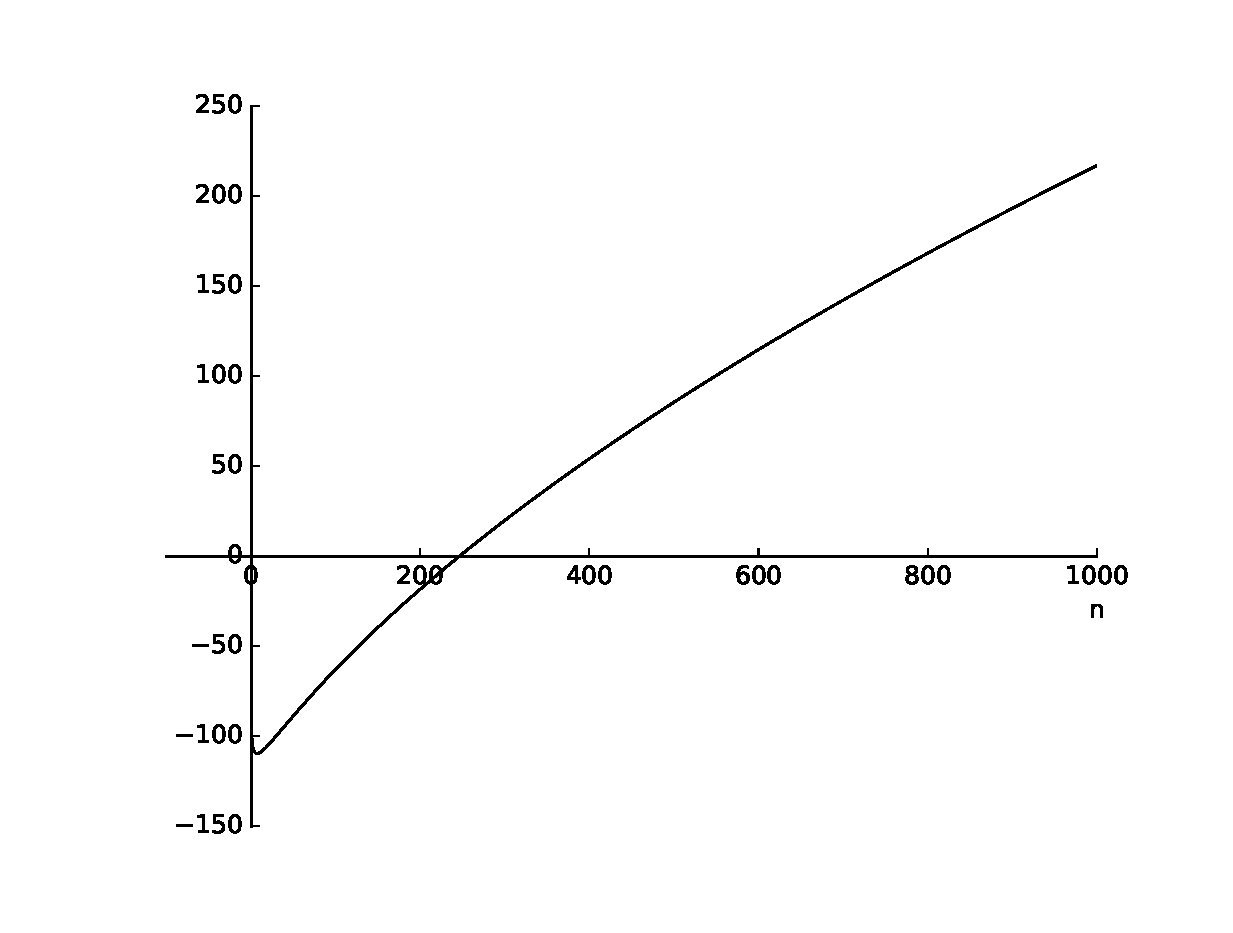
\includegraphics[scale=.25]{intro/sign_size}
%	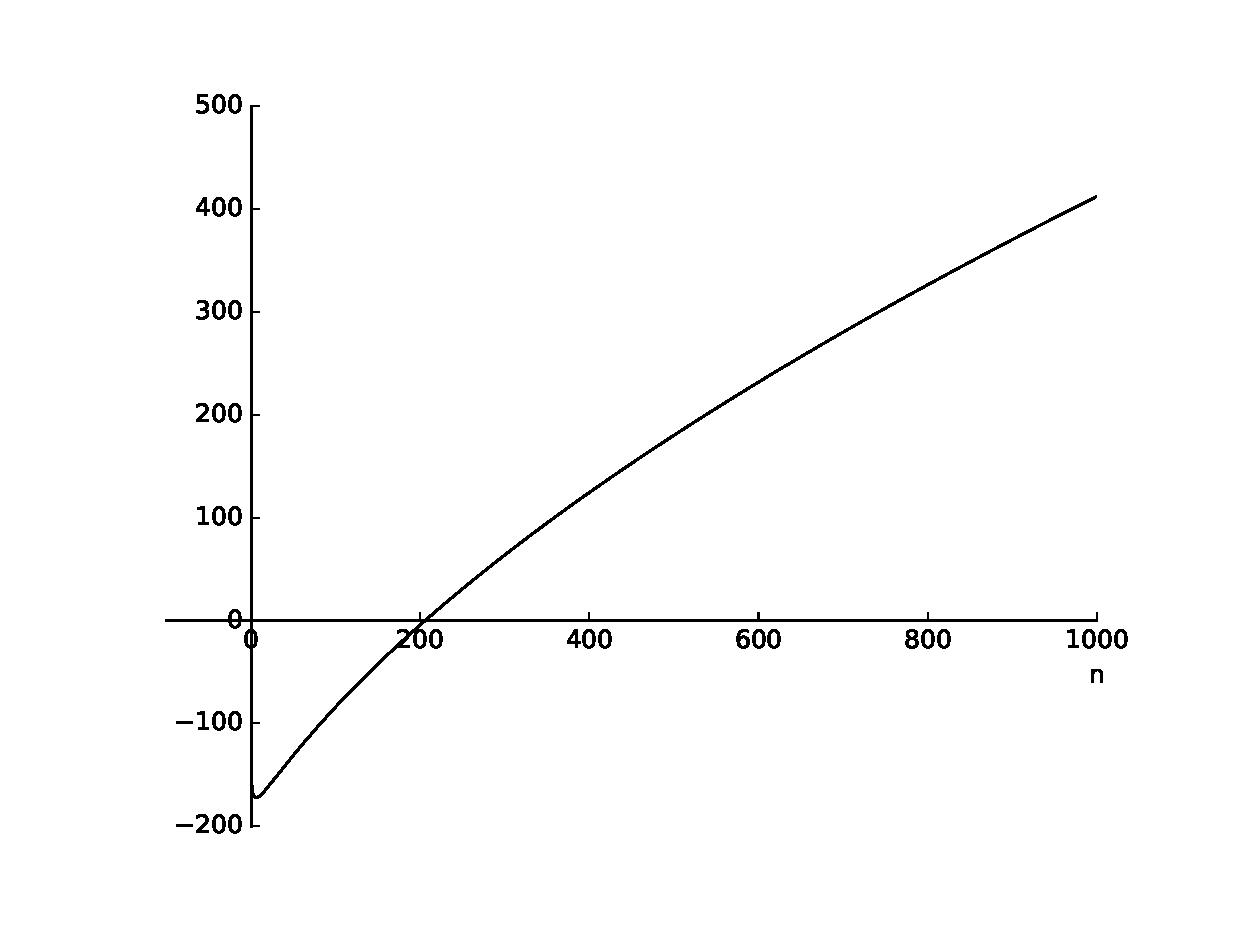
\includegraphics[scale=.25]{intro/sign_time}
%	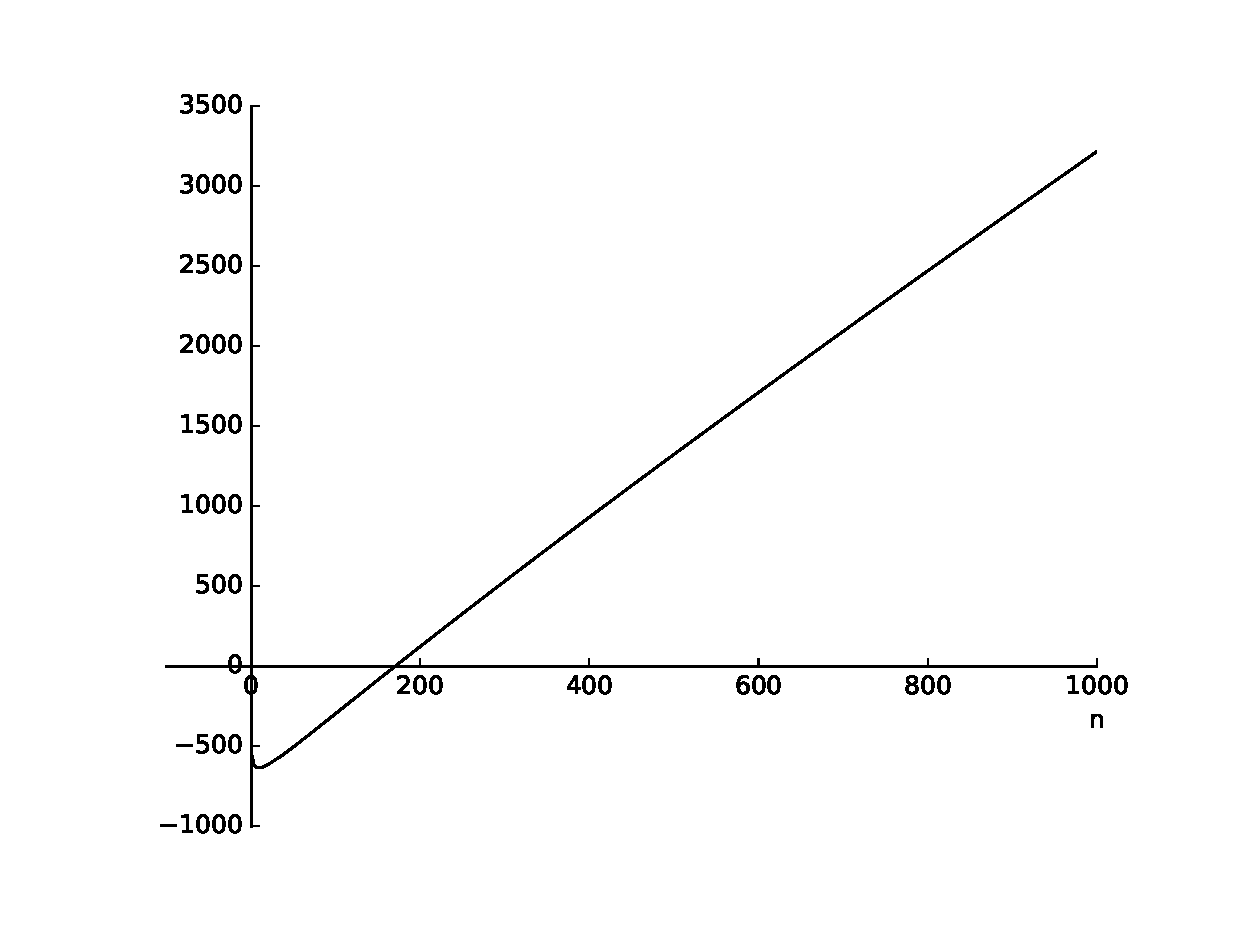
\includegraphics[scale=.25]{intro/ver_time}
%\end{figure}